\documentclass{standalone}
\usepackage{fontawesome}
\usepackage{tikz}
\usetikzlibrary[arrows.meta, graphs, positioning, quotes]

\begin{document}

  \begin{tikzpicture}
  [
  auto=right,
  block/.style={rectangle,draw=white,fill=black!30,minimum width=10ex,minimum height=4ex},
  smblock/.style={block, minimum width=6ex},
  ssmblock/.style={block, minimum width=3ex},
  sharrow/.style={shorten <=.5ex, shorten >=.5ex, >={Stealth[round]}, semithick},
  pre/.style={<-, sharrow},
  post/.style={->, sharrow}
  ]
  \small

  \node[align=center, inner sep=0pt] (file) {
  {\Large \faFileO}\\
  \texttt{.edf}
  };
  \node[block, fill=black!50, right=of file, xshift=4ex] (raw) {}
  edge[pre, "read raw"] (file);

  \node[block, right=of raw, xshift=4ex, minimum width=8ex] (resampled) {}
  edge[pre, "resample"] (raw);
  \node[smblock] at (resampled) {};

  % \node[minimum size=0pt, inner sep=0pt, right=of resampled, xshift=6ex] (preclips) {}
  % edge[shorten >=.5ex, "extract clips"] (resampled);
  % \node[smblock, above right=of preclips] {} edge[pre, shorten >=0ex] (preclips);
  % \node[smblock, below right=of preclips] {} edge[pre, shorten >=0ex] (preclips);
  \node[smblock, right=of resampled, xshift=8ex] (clip) {}
  edge[pre, "extract clip", pos=.4] (resampled.center);

  \node[right=of clip, xshift=9ex] (win_center) {}
  edge[pre, "windowing", pos=.6, shorten <=2.5ex, dashed] (clip);
  \draw[every node/.style=ssmblock] (win_center)
  node at +(-1.5ex,1.5ex) {}
  node at +(-.5ex,.5ex) {}
  node at +(.5ex,-.5ex) {}
  node at +(1.5ex,-1.5ex) {}
  ;

  \node[xshift=-3em, yshift=-6ex] (saved) at (resampled) {\Large \faFileZipO}
  edge[<->, >={Stealth[round]}, semithick, dotted, "save/load", bend right=45] (resampled.south);

  \end{tikzpicture}
\end{document}